%----------------------------------------------------------------------------
\chapter{Technologies}

I worked using tools from the JVM-ecosystem, focusing on the problem description's key values, modernity, compatibility and portability. As such, I avoided using deprecated programming structures and unstable dependencies wherever possible.

\section{Kotlin \raisebox{-1ex}{\hspace{1cm}
\includegraphics[height=8mm, keepaspectratio]{images/kotlin_logo.png}}}

Kotlin is a multiplatform, statically typed, multi-paradigm programming language. Its specification is publicly accessible and updated regularly by JetBrains employees.~\cite{KotlinSpec} The first prototype was release in 2011, and the code was open sourced just a year later. The first full release of the language was published in 2016; since 2017, Android officially supports the it, and Android development has been code-first since 2019.~\cite{KotlinPast}

Most of its popularity can be attributed to its intuitive syntax and near-perfect compatibility with JVM\footnote{JVM: \@Java Virtual Machine, a fully specified runtime currently owned by Oracle, mainly intended to run programs written in Java}. Any Java code can be referenced in a Kotlin program, allowing the use of countless Java community libraries. There is no restriction on the ratio of source files written in the two languages. It is worth noting however, that this compatibility is unidirectional -- Java code can not call Kotlin code.

Finished programs go through compile and optimisation phases before they are turned into executable applications or libraries. Binaries made with Kotlin's compiler have near-identical performance to their traditional JVM counterparts. There are non-JVM compile targets as well:
\begin{itemize}
    \item Kotlin/Native (Stable since 2023, provides native solutions for many operating systems without the need for a virtual machine)
    \item Kotlin/JS (programs are compiled to JavaScript, creating an interpreted codebase from compile-ready one; ideal for web browsers)
\end{itemize}

The language's code structure is simple, easy to understand and quick to write. A lot of the frustrating syntactic and technical elements from Java were skipped or built around -- I'll show examples for this and the functional paradigm's possibilities in code sections.

I used the newest (2.0.21) version for my thesis through JetBrains' own integrated developer environment, IntelliJ Idea. I targeted the Oracle OpenJDK distribution's 23rd main version. The program guarantees compatibility with past versions until 21 LTS\footnote{Long Term Support, in software development, a publisher's pledge to provide longer-lasting, multi year support for a release}, released in September 2023 -- this version loses support in 2028.~\cite{JavaRoadmap}

\section{OpenGL \raisebox{-1ex}{\hspace{1cm}
\includegraphics[height=8mm, keepaspectratio]{images/opengl_logo.png}}}

Popular low-level graphical library, capable of addressing the current screen down to the pixel level. It was first published in 1992, the newest version is 4.6, dating back to 2017 -- this is the single exception from my goals of using the latest tech.~\cite{OpenglHistory} OpenGL can be praised for its robustness and widespread support, the necessary graphics functions can be accessed on any operating system and by using nearly any programming language. Applications following the OpenGL standard can be expected to look identical on any system running it (provided the necessary dependencies are installed).

\section{libGDX \raisebox{-0.1ex}{\hspace{1cm}
\includegraphics[height=6mm, keepaspectratio]{images/libgdx_logo.png}}}

LibGDX got the name from its multiple use cases: it's a "game development" and "effects" library for Java-based projects. It provides helper functions to make OpenGL operations callable in a JVM-idiomatic way, making it surprisingly easy to adjust graphics code to the style of the rest of the application.

Its predecessor was meant to aid the display of Android applications specifically. In 2010, the code was open sourced, creating the community-focused development of today.~\cite{LibgdxHistory} The current version number is 1.13.0. Created games and apps can be presented on desktop environments (Windows, macOS, Linux), mobile operating systems (Android, iOS) and even in most web browsers.

\section{Exposed {\hspace{1cm}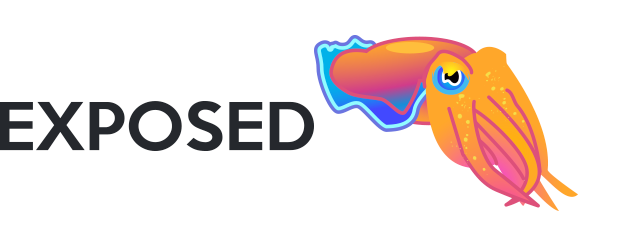
\includegraphics[height=8mm, keepaspectratio]{images/exposed_logo.png}}}

Databases, specifically SQL\footnote{Structured Query Language, a domain-specific language used in the management of relational databases} have very old roots. Although the past decade saw many improvements - mainly with the release of developer-friendly tools - the standard's 40 years long history still strongly affects present-day programs.


The language's dialects are similar to regional accents, in a linguistic sense; a "speaker" of one variant may understand most or all other types, but that doesn't mean that they have the ability to correctly "express" themselves when using other types. There are multitudes of ORM\footnote{Object Relational Mapping, a technique intended to transform database records and in-memory objects into one another} libraries intended to bridge this gap. The most well-known ones include Hibernate for Java, EntityFramework for \.NET/\texttt{C\#}, and Active Record used in Ruby on Rails applications. The newly preferred Kotlin solution is Exposed, built mainly on JDBC (Java Database Connectivity). The library reflects Kotlin's philosophy of developer freedom -- data can be accessed in a classic object oriented manner, or through a custom language highly reminiscent of raw SQL.~\cite{ExposedDocs}


Portability is endorsed with database-agnosticism. Switching between supported database engines only requires changing a few configuration values -- this allows releasing our app with one of many implementations, from SQLite (popular on mobile) to Oracle Database (intended for multiple tenants and a highly distributed workflow).

% TODO
\section{Ktor {\hspace{1cm}
\includegraphics[height=8mm, keepaspectratio]{images/ktor_logo.png}}}

Ktor is a Kotlin-based framework for creating asynchronous 